\documentclass[11pt,a4paper]{article}


\usepackage[utf8]{inputenc}
\usepackage{amsmath}
\usepackage{amsfonts}
\usepackage{amssymb}
\usepackage{indentfirst}
\usepackage{graphicx}
\usepackage[sorting = none]{biblatex}

\addbibresource{bibliography.bib}

\begin{document}



In 1916 Einstein published his General theory of relativity which explained that the two bodies orbiting each other would not be in the same orbit all the time. Instead the bodies lose energy and in doing so emit gravitational waves. But there was no practical evidence for this explanation. As for many years nobody was successful in observing the gravitational waves.\\


Several years later, in 1974\cite{Ligo} the first evidence of gravitational waves was deduced through the motion of the double neutron star system PSRB1913+16. In this system one of the star is a pulsar which emits electromagnetic pulses at radio frequencies precisely at regular intervals as it rotates. Russell Hulse and Joseph Taylor discovered this binary pulsars also noticed that the frequency of pulses shortened and the stars were gradually spiraling towards each other with an energy loss which is closely equal to the energy predicted to be radiated by gravitational waves. For this discovery, Hulse and Taylor were awarded the Nobel Prize in Physics in 1993.\cite{Lommen_2015}\\


 Further observations of the binary pulsar and other multiple systems also agree with the General theory of Relativity to high precision. This evidence of gravitational waves is considered as the first indirect evidence of gravitational waves. 
 
 
 
 
 \begin{figure}[htp]
    \centering
    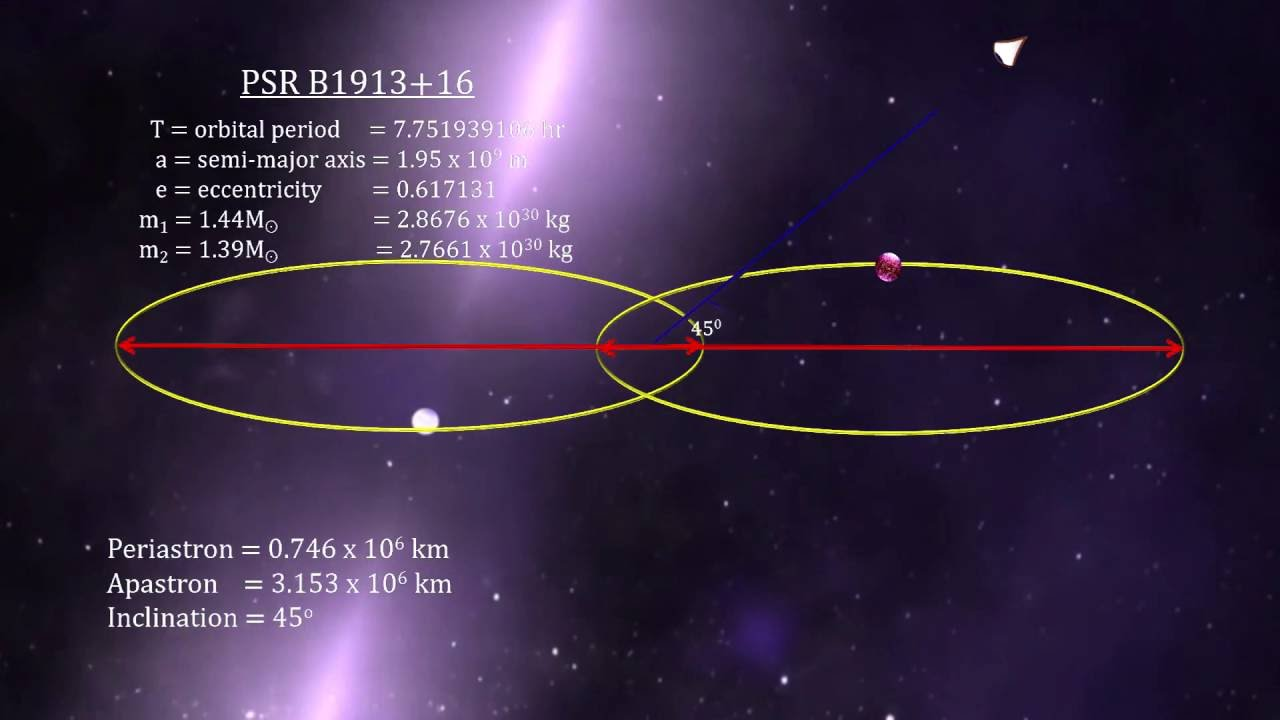
\includegraphics[width=6cm]{PSR-B191316}
    \caption{Binary pulsar PSR B1913+16}
    Source:\url{https://www.astroblogs.nl/wp-content/uploads/2014/03/PSR-B191316.jpg}
    \label{fig:pulsar}
    
\end{figure}


 
 
 
 
 
 
 
 
 
 
 
 
 
 \printbibliography
  
\end{document}